
\subsection*{Neues File Öffnen}
Beim Starten der Applikation wird ein leeres Fenster mit einem \textit{Load File} Button angezeigt. Betätigt man diesen Button, öffnet sich ein Dialogfenster, in dem der Benutzer ein \textit{.txt} File auswählen und öffnen kann. 

\begin{figure}[h!]
    \centering
    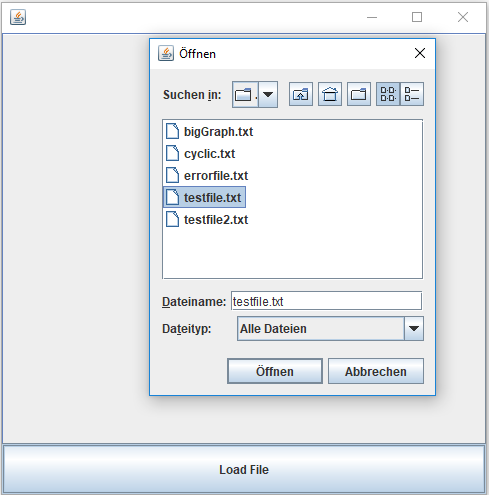
\includegraphics[width=.4\textwidth]{images/loadFile.png}
\end{figure}

Der \textit{Load File} Button ist auch noch dann sichtbar, wenn bereits Graphen geladen wurden. Öffnet man weitere Text Files, werden diese entsprechend in neuen Tabs geladen.

Ist das File kein Graph im Sinne unseres Eingabeformats oder ist der Graph nicht azyklisch, so wird eine Fehlermeldung ausgeben.

\subsection*{User Interface}

Hat der Benutzer einen gültigen Eingabegraphen ausgewählt und geöffnet, so stehen im mehrere Möglichkeiten zur Auswahl:

\begin{enumerate}
    \item[Anpassen der Fenstergrößen:] Alle Fenster können in ihrer Größe angepasst werden. Der Balken, der textuelle und graphische Ansicht der Graphen trennt, ist hierbei nur verschiebbar, wenn die Mindestgrößen der beiden Seiten nicht unterschritten werden.
   Das Panel, das die Steuerungselemente enthält kann per \textit{drag and drop} aus dem Fenster heraus- oder wieder hineingezogen werden.
    
    \item[Editieren des Graphen:] Auf der linken Seite des Fensters wird der Inhalt der geöffneten Textdatei angezeigt. Der Text kann modifiziert werden und die Änderungen durch das Klicken des \textit{Safe/Reload} Buttons gespeichert werden. Hierbei wird außerdem die Anzeige des Graphen neu geladen, so dass die vorgenommenen Änderungen sichtbar werden. 
    
    \textbf{Achtung! Erzeugt man hierbei einen ungültigen oder zyklischen Graphen, kann dies nur geändert werden, indem man außerhalb der Applikation die Datei öffnet und korrigiert!}
    
    \item[Graphen neu laden:] Den Knoten im Graphen werden zunächst Zufallskoordinaten zugewiesen, Dies kann dazu führen, dass sich Knoten beispielsweise überschneiden oder an einem Punkt häufen. Ist dergleichen der Fall, bietet es sich an den \textit{Safe/Reload} Button zu betätigen. Hierbei werden den Knoten neue Zufallskoordinaten zugewiesen.
    
    \item[Weitere Graphen öffnen:] Um weitere Graphen in neuen Tabs zu öffnen, kann der Benutzer den \textit{Load File} Button betätigen.
    
    \item[Justierungen vornehmen:] Die GUI stellt drei Slider bereit, die es dem Benutzer erlauben die Darstellung des Graphen und die Animation des Algorithmus anzupassen. Der \textit{Step Size} Slider legt fest, wie viele Berechnungsschritte auf ein mal ausgeführt werden sollen. Über Textfeld neben dem \textit{Step Size} Slider kann die Selbe Angabe gemacht werden. 
    
    Der \textit{Speed} Slider definiert wie schnell sich die Knoten in der Animation bewegen.
    
    Der \textit{Size} Slider setzt die Größe der Knoten fest und damit auch die Größe des Labels im Knoten.
    
    \item[Anzeige Speichern:] Per Rechtsklick auf die rechte Seite des Fensters (die den Graphen anzeigt) kann der Benutzer einen Snapshot der aktuellen Anzeige speichern.
    
    \item [Animation Starten/Stoppen:] Durch Drücken des \textit{play} Buttons kann der Benutzer die Animation starten, die entsprechend seiner Justierungen den Algorithmus auf den Graphen Ausführt. Durch Drücken auf den \textit{Pause} Button wird die Animation im aktuellen Schritt unterbrochen. 
    
    \item[Zurücksetzen:]Wird der \textit{Reset} Button gedrückt, so begeben sich die Knoten wieder zu ihren Ursprungspositionen und die Animation kann erneut gestartet oder der Algorithmus schrittweise verfolgt werden.
    
    \item[Schrittweises Ausführen:] Die Button \textit{Jump Forward} und \textit{Jump Backward} springen jeweils um so viele Berechnungsschritte vor oder zurück, wie über den \textit{Step Size} Slider angegeben wurde.
    
    
\end{enumerate}


\begin{figure}[ht!]
    \centering
    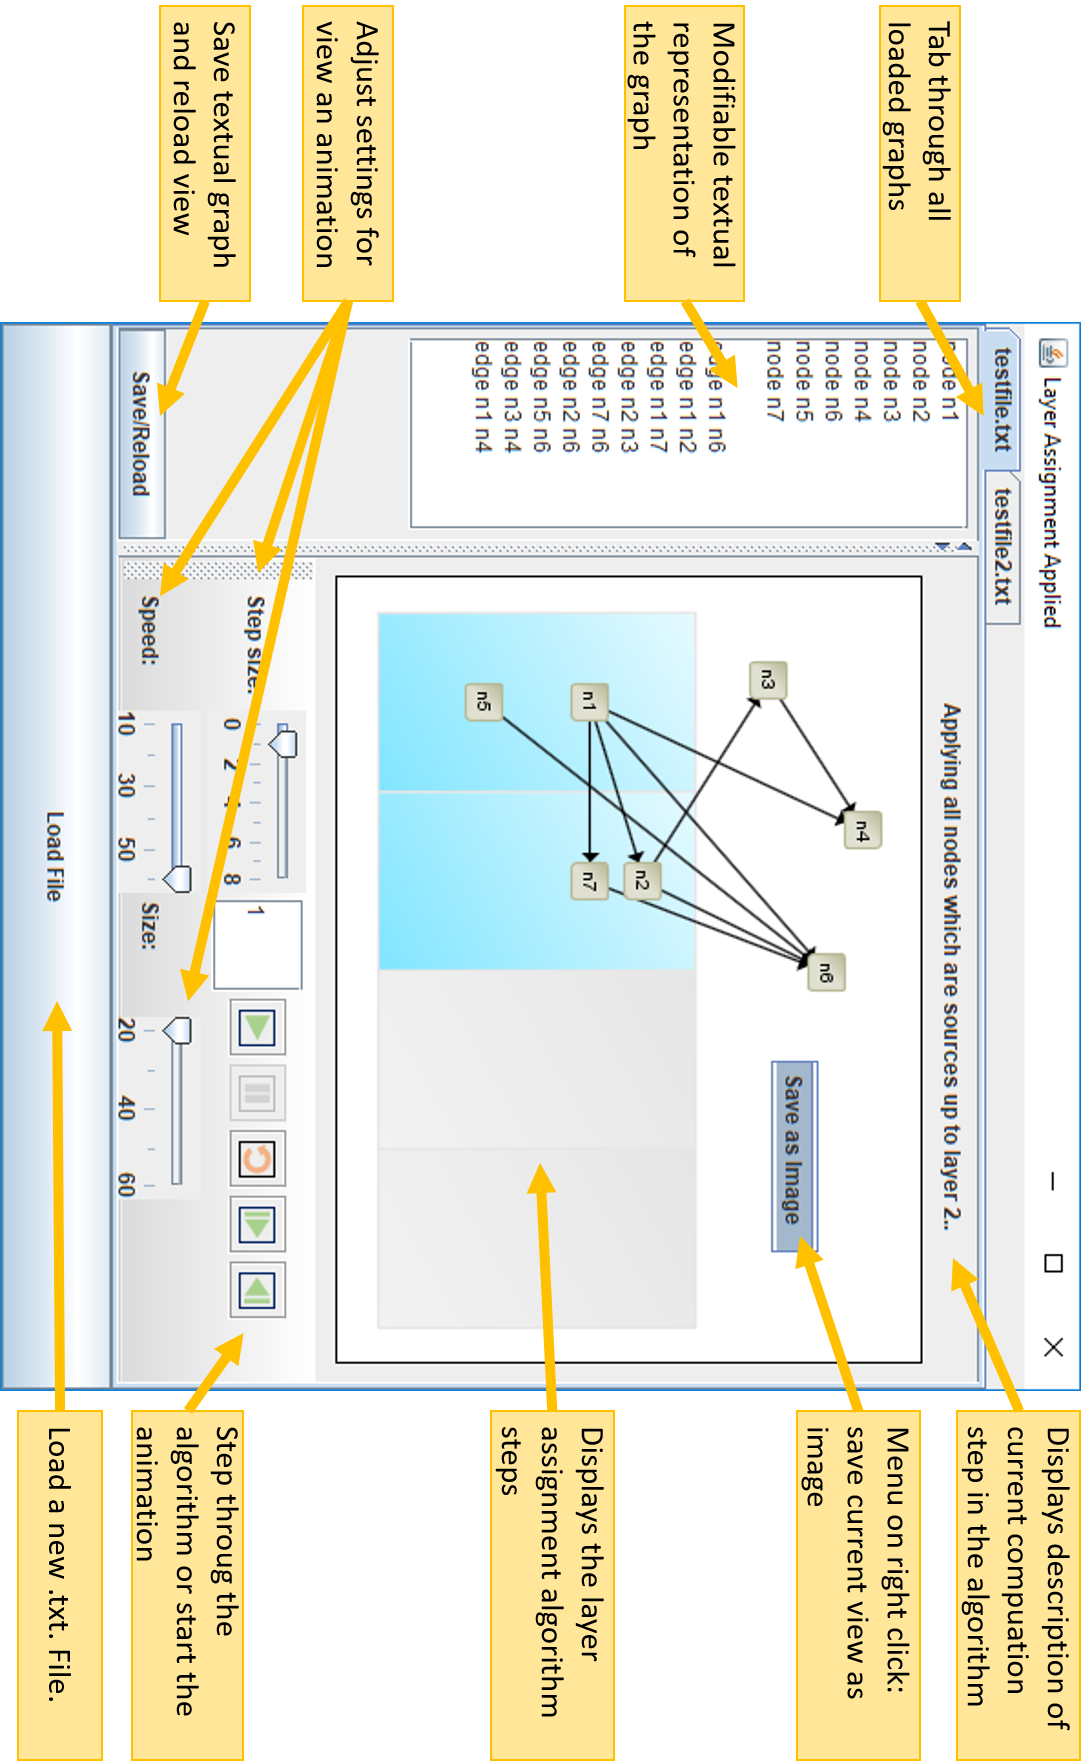
\includegraphics[width=\textwidth ]{images/toolGuide.png}
\end{figure}
